% ================================================================
\section{Results and Discussion}
% ================================================================

\subsection{Evaluation Protocol}

We evaluate using HumanEval, which comprises 164 hand-authored Python
programming problems. Each problem gives a function signature and we
generate the body with greedy decoding (a single deterministic sample
per problem, up to 512 new tokens), then report pass@1: the fraction
of problems whose generated body passes all hidden unit tests. The
prompt is the bare function signature in a zero-shot setting, matching
how a local autocompletion endpoint queries the model rather than the
few-shot, chat-formatted protocol used in the model's own technical
report. We evaluate two checkpoints under identical conditions:
(i) the unmodified Qwen2.5-Coder-1.5B base model (baseline), and
(ii) the merged fine-tuned model after one epoch of QLoRA training.
Because decoding is deterministic, the only source of uncertainty is
the finite 164-problem set; we report 95\% Wilson confidence intervals
on each proportion (the range of pass@1 values consistent with the
observed sample at 95\% confidence).

\subsection{Quantitative Results}

Table~\ref{tab:results} reports pass@1 for both checkpoints with 95\%
Wilson intervals. Fig.~\ref{fig:passatk} visualises the comparison.
The fine-tuned model reaches 42.68\% with a 95\% confidence interval
of [35.4, 50.3], compared to 10.98\% [7.1, 16.7] for the baseline;
the intervals denote the plausible range for the true pass@1 given
164 test problems. The intervals do not overlap, so the gain of 31.7
percentage points is statistically distinguishable under this
zero-shot protocol. Both checkpoints are evaluated under identical
conditions, so this gain is a direct measure of the fine-tuning
contribution in our deployment-faithful setting.

\begin{table}[htbp]
  \centering
  \caption{HumanEval Pass@1 (zero-shot, greedy, 95\% Wilson CI)}
  \label{tab:results}
  \begin{tabular}{lccc}
    \toprule
    \textbf{Model} & \textbf{Pass@1} & \textbf{95\% CI} & \textbf{Correct / 164} \\
    \midrule
    Qwen2.5-Coder-1.5B (baseline) & 10.98\% & [7.1, 16.7] & 18 \\
    Completus Python (fine-tuned)  & 42.68\% & [35.4, 50.3] & 70 \\
    \midrule
    \textbf{Improvement} & \textbf{+31.70 pp} & --- & \textbf{+52} \\
    \bottomrule
  \end{tabular}
\end{table}

\begin{figure}[t]
  \centering
  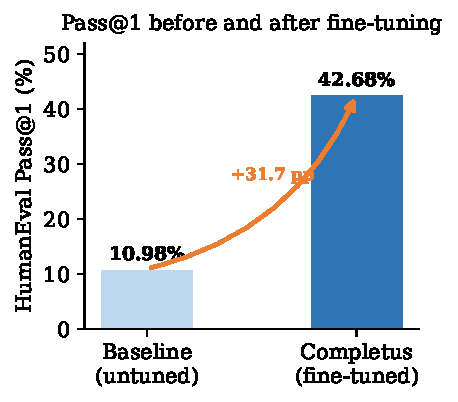
\includegraphics[width=0.55\textwidth]{fig_passatk.pdf}
  \caption{Pass@1 on HumanEval (164 problems). The fine-tuned model
  (42.68\%) outperforms the baseline (10.98\%) by 31.7 percentage
  points after one epoch of QLoRA fine-tuning on CodeSearchNet Python.}
  \label{fig:passatk}
\end{figure}

\subsection{Qualitative Examples}

Both the \texttt{python-coder} and \texttt{go-coder} Ollama models,
queried with \texttt{factorial} as the prompt, return syntactically
valid and semantically correct implementations:

\noindent\begin{minipage}{\linewidth}
\begin{lstlisting}[language=Python, title=Python]
def factorial(n):
    # n! = n * (n-1) * (n-2) * ... * 1
    if n == 0:
        return 1
    else:
        return n * factorial(n - 1)
\end{lstlisting}
\end{minipage}

\noindent\begin{minipage}{\linewidth}
\begin{lstlisting}[language=Go, title=Go]
func factorial(n int) int {
    // factorial of n
    if n == 0 {
        return 1
    }
    return n * factorial(n-1)
}
\end{lstlisting}
\end{minipage}

\subsection{Comparison with Prior Work}

Table~\ref{tab:comparison} places our result alongside HumanEval
pass@1 scores reported by the original authors of comparable open code
models. These published figures are obtained under each model's own
evaluation protocol (typically few-shot or greedy chat-format decoding)
and are therefore not directly comparable to our stricter zero-shot
setting; the table is intended as broad context rather than a
controlled head-to-head benchmark.

\begin{table}[htbp]
  \centering
  \caption{HumanEval Pass@1 as Reported by Original Authors. Settings
  differ across rows and are not directly comparable.}
  \label{tab:comparison}
  \begin{tabular}{lrrl}
    \toprule
    \textbf{Model} & \textbf{Params} & \textbf{Pass@1} & \textbf{Source} \\
    \midrule
    CodeLlama-Base~\cite{Roziere2023CodeLlama}    & 7B    & 31.7\% & \cite{Guo2024DeepSeek}, Table~3 \\
    StarCoderBase~\cite{Li2023StarCoder}          & 15.5B & 31.7\% & \cite{Guo2024DeepSeek}, Table~3 \\
    DeepSeek-Coder-Base~\cite{Guo2024DeepSeek}   & 1.3B  & 34.8\% & \cite{Guo2024DeepSeek}, Table~3 \\
    \midrule
    \textbf{Completus (ours)} & \textbf{1.5B} & \textbf{42.68\%} & \textbf{Zero-shot, local} \\
    \bottomrule
  \end{tabular}
\end{table}

Our fine-tuned model reaches 42.68\% under a strict zero-shot
evaluation in which the untuned base model, measured by us under
identical conditions, scores only 10.98\% (Section~\ref{ssec:disc}).
Completus thus delivers competitive pass@1 in this deployment-faithful
regime while running entirely locally on consumer hardware.

\subsection{Discussion}
\label{ssec:disc}

\paragraph{Baseline measurement.}
We measure the untuned base model at 10.98\% pass@1 under our protocol,
which uses zero-shot prompting with raw function signatures rather than
a few-shot, chat-formatted prompt, matching how a local autocompletion
endpoint queries the model. Both checkpoints are evaluated under
identical conditions, so the 31.7\,pp improvement is a valid measure
of the fine-tuning contribution.

\paragraph{Effect of fine-tuning.}
One epoch of instruction-style fine-tuning on CodeSearchNet teaches
the model to generate function bodies in the plain-Python format
expected by HumanEval, consistent with the finding by Weyssow et
al.~\cite{Weyssow2023PEFT} that LoRA adapters rapidly adapt pretrained
code models to narrower formats and domains.

\paragraph{Limitations.}
We evaluate only Python on HumanEval; a dedicated Go benchmark (e.g.,
HumanEval-X) would quantify cross-language transfer. HumanEval
measures correctness on short, self-contained functions and does not
capture multi-file, context-dependent completion scenarios. We cap
pipeline input at 50,000 functions per language and do not study how
a larger input or different filter thresholds would affect the
trade-off between data quality and training set size.
